%% Essa classe foi adaptada do formato de conferências da ACM
\documentclass[sigconf]{educomp}

%Na versão final remover as tags review e anonymous
%\documentclass[sigconf]{educomp}

\renewcommand\refname{Referências}

%%% REMOVER ESSE PACOTE PARA A VERSAO FINAL %%%%%%%%%%%%%%%%%
\usepackage{lipsum}

%% Não altere essas informações. Elas serão enviadas aos autores após ao aceite no ato da publicação dos anais.

\copyrightyear{2026}
\acmYear{2026}
\setcopyright{sbcpt} %%% Para artigos escritos em inglês, troque para sbcen
%alterar o nome do evento, data e local do evento para a versão correta
\acmConference[EduComp'26]{Simpósio Brasileiro de Educação em Computação}{Abril 22-27, 2024}{São Paulo, São Paulo, Brasil (On-line)}
\acmBooktitle{Simpósio Brasileiro de Educação em Computação (EduComp '24), Abril 22-27, 2024, São Paulo, São Paulo, Brasil (On-line)}

%%% REMOVER A PRÓXIMA LINHA PARA ARTIGOS ESCRITOS EM INGLÊS
\usepackage[brazil]{babel}

%%%%%%%%%%
\nocite{*}
\begin{document}

%%% TITULO
\title[Título curto]{EduComp 2026}


%Autores
\author{Bruna Luisa dos Santos, Maria Eduarda Menezes, Yago Welsing Pereira}
\email{{brunaluisacosareis, dolivr.br, yagowelsing}@gmail.com} 
\affiliation{%
  \institution{The Fab Four, Manchester, UK}
}

%% By default, the full list of authors will be used in the page
%% headers. Often, this list is too long, and will overlap
%% other information printed in the page headers. This command allows
%% the author to define a more concise list
%% of authors' names for this purpose.
%\renewcommand{\shortauthors}{-}

\newcommand{\showDOI}[1]{\unskip}


%%%%% ABSTRACT %%%%%%%%%%%%%%%%%%%%%%%%%%%%%%%
\begin{abstract}

Este trabalho utiliza técnicas de Mineração de Dados e algoritmos de classificação e predição para personalizar a jornada acadêmica de estudantes de graduação, visando reduzir o tempo de conclusão do curso. Através da análise de variáveis como o desempenho em disciplinas e o histórico de reprovações, a pesquisa busca mapear o perfil de cada aluno. Ao comparar esses dados com o histórico de alunos que já concluíram o curso com sucesso, o sistema propõe o fluxo de disciplinas mais compatível com as facilidades do estudante, ajudando a superar dificuldades e potencializar o aproveitamento acadêmico.


\end{abstract}

%%%% PALAVRAS-CHAVE %%%%%%%%%%%%%%
\keywords{Knn, K-Means, Naive Bayes, tutor inteligente, inteligência artificial, educação, desempenho acadêmico, mineração de dados educacionais, otimização de tempo de formação} % germane load

%%
%% This command processes the author and affiliation and title
%% information and builds the first part of the formatted document.
\maketitle

% Arquivo da Introdução
\section{Introdução}

De acordo com \citet{bispo2020tecnologias}: 

\begin{quote}
Embora Informática na Educação (IE) e Educação de Computação (EC) partilhem muitos elementos metodológicos, epistemológicos, contextos de pesquisa e em alguns casos até objetivos de pesquisa convergentes, a EC distingue-se como área
de pesquisa específica por sua \emph{raison d’être}: a busca do entendimento profundo de fenômenos complexos e processos envolvidos no ensino e aprendizado de computação \cite{malmi2019computing}. Além disso, enquanto as TEC e a IE pressupõem o emprego de um artefato tecnológico no processo de ensino e/ou aprendizagem, a EC pode utilizar-se ou não de tais artefatos para o ensino dos processos de computação. Assim como a Ciência da Computação ainda pode ser considerada uma ciência relativamente nova e em desenvolvimento, a EC ainda encontra-se em um estado de maturação \cite{malmi2019computing}. Ainda que a maioria das teorias utilizadas para o ensino de computação seja adaptada de outras áreas de tecnologia (como a engenharia, matemática ou ciências de forma geral), ou de teorias de educação ou psicologia da educação de forma mais ampla \cite{malmi2014theoretical}, já é possível observar o advento de teorias e práticas pedagógicas próprias \cite{malmi2019computing} com um crescente suporte empírico \cite{malmi2014theoretical}
\end{quote}


\lipsum[3-10]

% Arquivo da Revisão da Literatura
\section{Trabalhos Relacionados}
A análise de dados aplicada à melhoria do desempenho acadêmico tem sido amplamente explorada na literatura, especialmente no contexto de Learning Analytics e Mineração de Dados Educacionais.

Na fase inicial deste trabalho, destacam-se como base teórica os estudos “Student Course Grade Prediction Using the Random Forest Algorithm: Analysis of Predictors' Importance” e “Analyzing Undergraduate Students' Performance Using Educational Data Mining”, que investigam o uso de técnicas de aprendizado de máquina para predição de desempenho acadêmico e identificação de fatores relevantes no progresso dos estudantes.

Essas abordagens fundamentam a análise e o tratamento dos dados dos discentes do curso de Ciência da Computação da UFRRJ, contribuindo para o treinamento do agente proposto. No entanto, diferentemente dos trabalhos mencionados, que se concentram predominantemente na predição de desempenho, este trabalho busca utilizar tais informações para apoiar a recomendação de disciplinas, com o objetivo de otimizar o tempo de formação dos estudantes.


% Arquivo da Metodologia
\section{Métodos}

\lipsum[5-10]



% Arquivo dos Resultados
\section{Resultados}

\lipsum[7-14]

% Please add the following required packages to your document preamble:
% \usepackage[normalem]{ulem}
% \useunder{\uline}{\ul}{}
\begin{table}[htb]
\label{tb:records}
\caption{Beatles Discography (UK)}
\begin{tabular}{llc}
\hline
\multicolumn{1}{c}{\textbf{Title}}    & \multicolumn{1}{c}{\textbf{Released}} & \textbf{Label}            \\ \hline
Please Please Me                      & 22 March 1963                         & Parlophone                \\
With the Beatles                      & 22 November 1963                      & Parlophone                \\
A Hard Day's Night                    & 10 July 1964                          & Parlophone                \\
Beatles for Sale                      & 4 December 1964                       & Parlophone                \\
Help!                                 & 13 August 1965                        & Parlophone                \\
Rubber Soul                           & 3 December 1965                       & Parlophone                \\
Revolver                              & 5 August 1966                         & Parlophone                \\
Sgt. Pepper's Lon. H. C. B. & 26 May 1967                           & Parlophone                \\
Magical Mystery Tour                  & 27 November 1967                      & Parlophone                \\
"The White Album"       & 22 November 1968                      & \multicolumn{1}{l}{Apple} \\
Yellow Submarine                      & 13 January 1969                       & \multicolumn{1}{l}{Apple} \\
Abbey Road                            & 26 September 1969                     & \multicolumn{1}{l}{Apple} \\
Let It Be                             & 8 May 1970                            & \multicolumn{1}{l}{Apple} \\ \hline
\end{tabular}
\end{table}

\lipsum[14-18]

\begin{figure}[t]
  \begin{center}
    %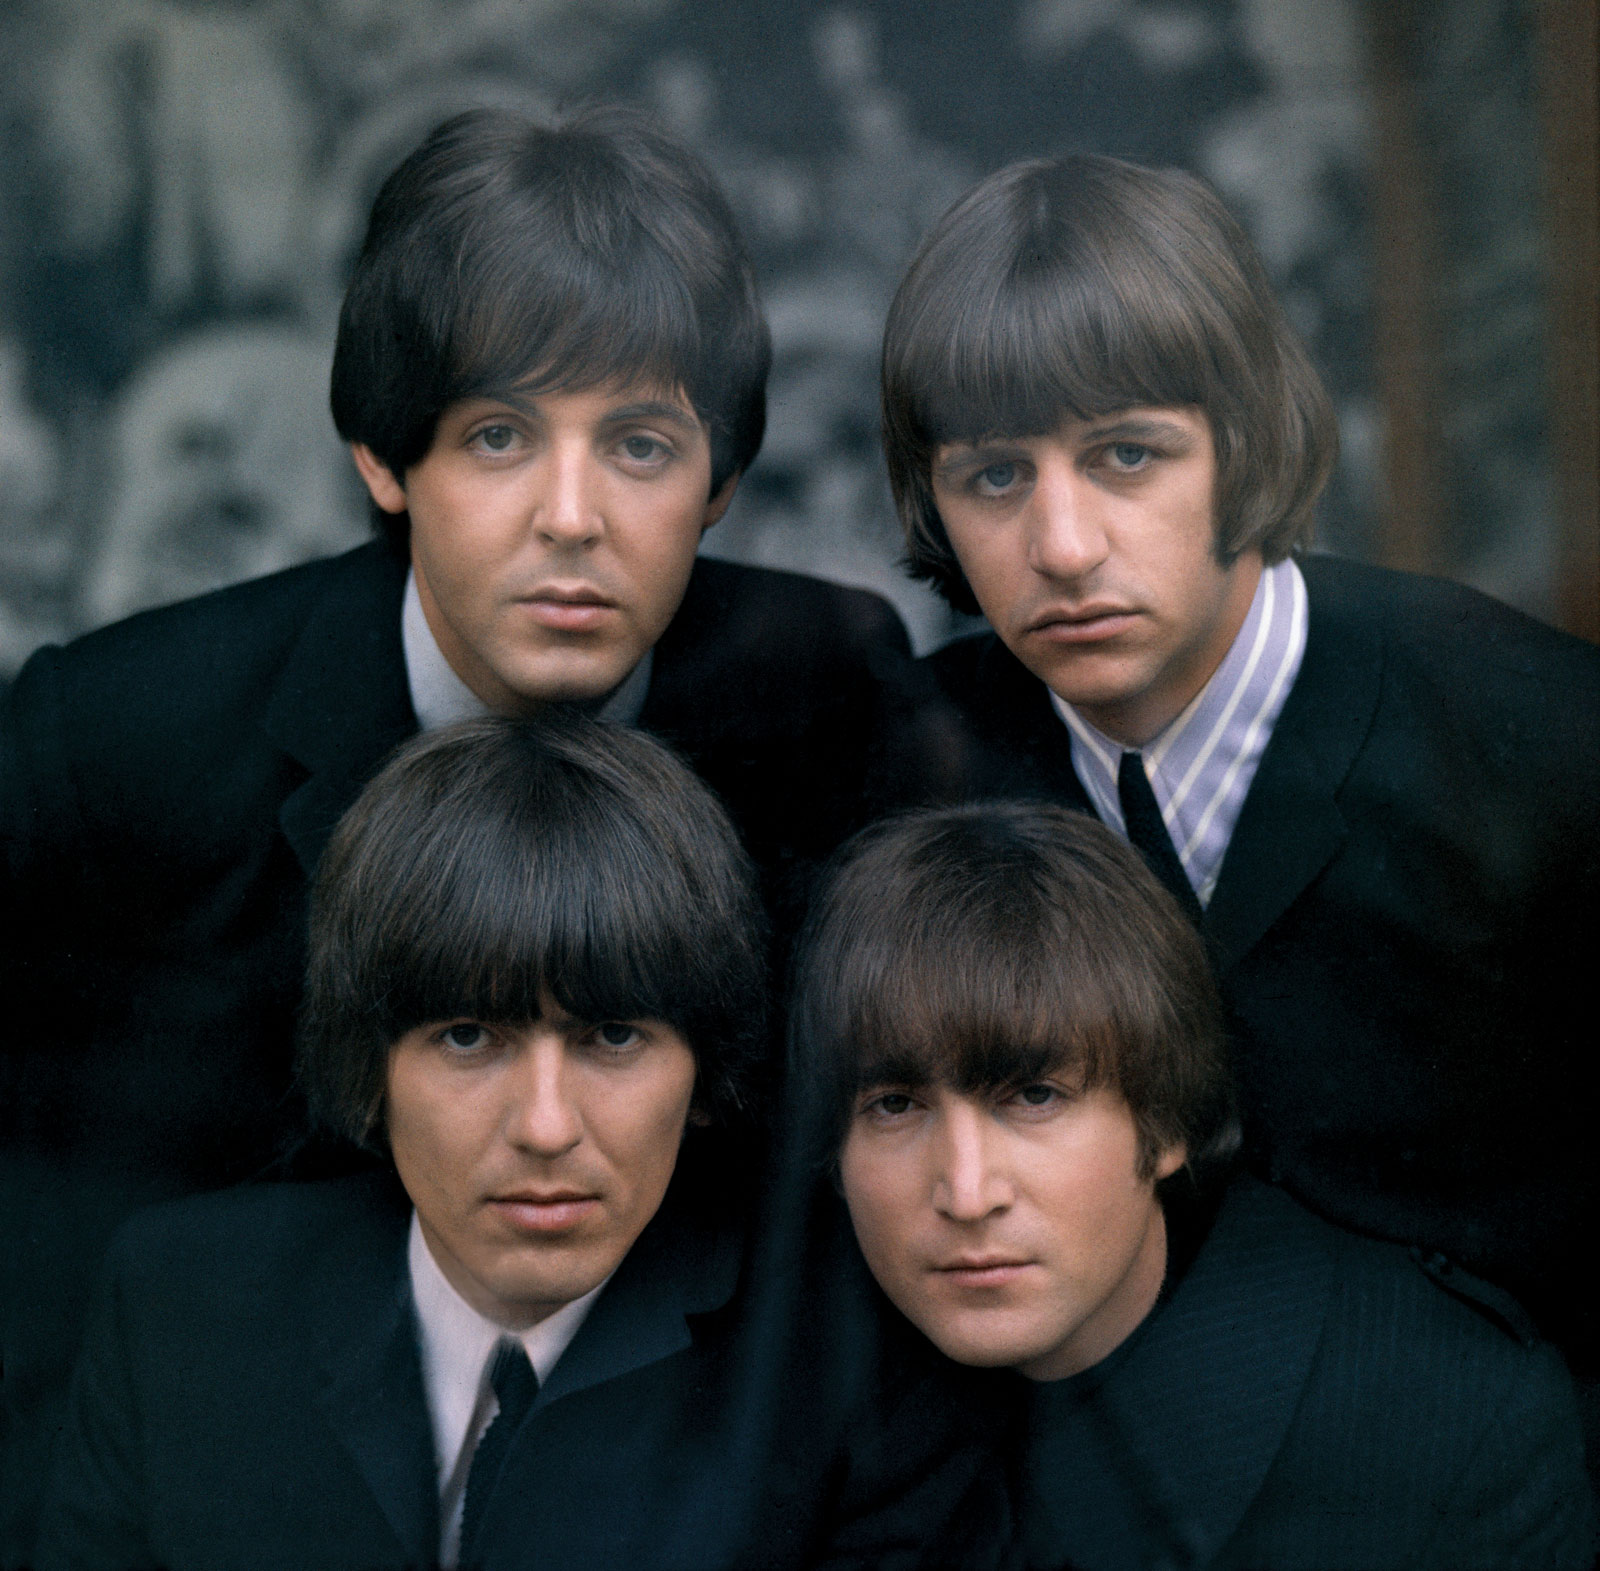
\includegraphics[width=\columnwidth]{Images/beatles.jpg}
    \caption{The Fab Four} 
    \label{fig:beatles}
  \end{center}
\end{figure}

\lipsum[18-20]



% Arquivo dos Discussao

\section{Discussão}

\lipsum[20-27] \cite{Goossens:1999:LWC:553897, Clarkson:1985:ACP:911891, KA:2001, KAGM:2001}

\subsection{Limitações}

\lipsum[27-29]





% Arquivo dos Discussao
\section{Considerações Finais}

\lipsum[29-30]

\subsection{Trabalhos Futuros}

\lipsum[31-32]

\bibliographystyle{ACM-Reference-Format}
\bibliography{references}
\nocite{*}
\end{document}